\chapter{Semiclassical Transport}
\section{Boltzmann Transport Equation}
In Chapter 2, we've discussed how to calculate the current with the Hamiltonian of the material. However, the brute force of solving this complicated problem is numerically inefficient. Therefore, a semiclassical way, which includes the quantum mechanical correction, is desired. The Fermi distribution can be written as \begin{equation}
    f_{k} = \frac{1}{1+e^{(E_{k}-\mu)/(k_{B}T)}} = \frac{1}{1+e^{(\frac{P^{2}}{2m}-\mu)/(k_{B}T)}}
\end{equation} Since $p = \hbar k$, the $f_{k}$ in general is shown in Fig. 4.1.
\begin{figure}[tbp]
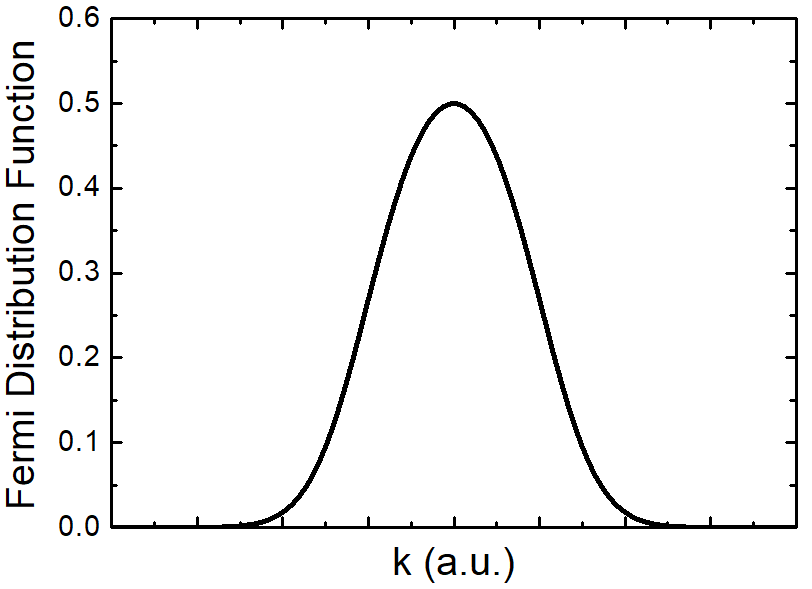
\includegraphics[width=0.4\textwidth]{figures/Fig4_1}
\centering
\caption{\small Fermi distribution function as a function of $k$.}
\end{figure}
The $f_{k}$ can be further extended into space-, momentum-, and time-dependence, i.e., \begin{equation}
    f_{k} = g(\overset{\rightharpoonup}{r}, \overset{\rightharpoonup}{p}, t)
\end{equation} where there are 7 dimensions (3 in space, 3 in momentum, and 1 in time). When applying the electric field $\overset{\rightharpoonup}{E}$, the Master equation says \begin{align}
    \frac{df_{k}}{dt}& = \sum_{k'}{S_{kk'}f_{k'}(1-f_{k})} - \sum_{k'}{S_{k'k}f_{k}(1-f_{k'})} + \frac{\partial f_{k}}{\partial t}\big|_{\overset{\rightharpoonup}{E}}\nonumber\\
    & \equiv \vec{S^{\text{OP}}}f_{k} + \frac{\partial f_{k}}{\partial t}\big|_{\overset{\rightharpoonup}{E}}
\end{align} From the Newton's law, we have \begin{equation}
    \overset{\rightharpoonup}{F} = m\overset{\rightharpoonup}{a} = \frac{d\overset{\rightharpoonup}{p}}{dt} = -e\overset{\rightharpoonup}{E}\Rightarrow\Delta p_{x} = -eE_{x}\Delta t
\end{equation} and \begin{equation}
    \Delta x = v_{x}\Delta t
\end{equation} if the electric field is only in the $x$-direction. Assume that the electric field does not perturb the shape of the $f$ after $\Delta t$. \begin{equation}
    f(\overset{\rightharpoonup}{r}, \overset{\rightharpoonup}{p}, t+\Delta t) = f(\overset{\rightharpoonup}{r}-v_{x}\Delta t, \overset{\rightharpoonup}{p}+eE_{x}\Delta t, t)
\end{equation} Apply the Taylor expansion to the Equation (4.6), we have \begin{equation}
    f_{0}+\frac{\partial f}{\partial t}\big|_{\overset{\rightharpoonup}{r}, \overset{\rightharpoonup}{p}, t}\Delta t = f_{0} + \frac{\partial f}{\partial \overset{\rightharpoonup}{r}}\big|_{\overset{\rightharpoonup}{r}, \overset{\rightharpoonup}{p}, t}(-v_{x}\Delta t) + \frac{\partial f}{\partial \overset{\rightharpoonup}{p}}\big|_{\overset{\rightharpoonup}{r}, \overset{\rightharpoonup}{p}, t}eE_{x}\Delta t
\end{equation} If the scattering $\vec{S^{\text{OP}}}$ is considered, then in general we have \begin{equation}
    \boxed{\frac{\partial f}{\partial t} = (\nabla_{r}f)\cdot(-\overset{\rightharpoonup}{v}) + (\nabla_{p}f)\cdot(e\overset{\rightharpoonup}{E}) + \vec{S^{\text{OP}}}f}
\end{equation} The above equation can be further simplified using the fact that \begin{equation}
    \nabla\cdot(f\overset{\rightharpoonup}{v}) = f\underbrace{(\nabla\cdot\overset{\rightharpoonup}{v})}_{=0} + \overset{\rightharpoonup}{v}\cdot(\nabla f)
\end{equation} where the first term at the right hand side is zero because there is no space-dependence in $\overset{\rightharpoonup}{v}$. Thus, the Equation (4.8) becomes \begin{equation}
    \boxed{\frac{\partial f}{\partial t} + \nabla\cdot(f\overset{\rightharpoonup}{v}) = e\overset{\rightharpoonup}{E}\nabla_{p}f + \vec{S^{\text{OP}}}f}
\end{equation} which is called the {\bf Boltzmann Transport Equation (BTE)}.
\section{Simplification of BTE}
Suppose we have a measurable $\vec{A}$ \begin{equation}
    \big<\vec{A}\big> = \sum_{k}{A_{k}f_{k}}
\end{equation} Multiplying $\sum_{k}{A_{k}}$ to the BTE, we have \begin{equation}
    \frac{\partial \big<\vec{A}\big>}{\partial t} + \nabla\cdot\sum_{k}{A_{k}f_{k}v_{k}} = \frac{e\overset{\rightharpoonup}{E}}{\hbar}\cdot\sum_{k}{A_{k}\nabla_{k}f} - \frac{\big<\vec{A}\big>-\big<\vec{A}\big>_{0}}{\big<\tau_{A}\big>}
\end{equation} where $\big<\tau_{A}\big>$ is the relaxation time as defined in the Equation (3.35), and we define \begin{equation}
    \overset{\rightharpoonup}{J_{A}} \equiv \sum_{k}{A_{k}f_{k}v_{k}}
\end{equation} \begin{align}
    G_{A}& \equiv \frac{e\overset{\rightharpoonup}{E}}{\hbar}\cdot\sum_{k}{A_{k}\nabla_{k}f}= \frac{e\overset{\rightharpoonup}{E}}{\hbar}\cdot\frac{V}{8\pi^{3}}\int_{-\infty}^{\infty}d^{3}kA_{k}\nabla_{k}f\nonumber\\
    & = \frac{e\overset{\rightharpoonup}{E}}{\hbar}\cdot\frac{V}{8\pi^{3}}\left[A_{k}\int_{-\infty}^{\infty}d^{3}k\nabla_{k}f-\int_{-\infty}^{\infty}\frac{dA_{k}}{dk}d^{3}k\int_{-\infty}^{\infty}d^{3}k\nabla_{k}f\right]\nonumber\\
    & = \frac{e\overset{\rightharpoonup}{E}}{\hbar}\cdot\frac{V}{8\pi^{3}}\left[fA_{k}\big|_{-\infty}^{\infty}-\int_{-\infty}^{\infty}d^{3}k(f\nabla_{k}A_{k})\right]\nonumber\\
    & = -\frac{e\overset{\rightharpoonup}{E}}{\hbar}\cdot\frac{V}{8\pi^{3}}\int_{-\infty}^{\infty}d^{3}k(f\nabla_{k}A_{k})\nonumber\\
    & = -\frac{e\overset{\rightharpoonup}{E}}{\hbar}\sum_{k}f_{k}(\nabla_{k}A_{k})
\end{align} \begin{equation}
    R_{A} \equiv \frac{\big<\vec{A}\big>-\big<\vec{A}\big>_{0}}{\big<\tau_{A}\big>}
\end{equation}
If $\boxed{A_{k} = -e}$, we have \begin{equation}
    \frac{\partial \big<\vec{A}\big>}{\partial t} = \frac{\partial}{\partial t}\sum_{k}{f_{k}(-e)} = -\frac{e\partial n}{\partial t}
\end{equation} \begin{equation}
    \nabla\cdot\overset{\rightharpoonup}{J_{k}} = \nabla\cdot\sum_{k}{(-e)f_{k}v_{k}} = \nabla\cdot\overset{\rightharpoonup}{J}
\end{equation} \begin{equation}
    G_{A} = -\frac{e\overset{\rightharpoonup}{E}}{\hbar}\sum_{k}f_{k}\nabla_{k}(-e) = 0
\end{equation} \begin{equation}
    \frac{1}{\big<\tau_{k}\big>}(k) = \sum_{k'}{\frac{S_{k'k}f_{k}(1-f_{k'})}{f_{k}-f_{k0}}\left[1-\frac{A_{k'}}{A_{k}}\right]} = 0\quad \text{since} \quad A_{k} = A_{k'} = -e
\end{equation} Therefore, we get the continuity equation from the BTE. \begin{equation}
    \boxed{e\frac{\partial n}{\partial t} = \nabla\cdot\overset{\rightharpoonup}{J}}
\end{equation}If $\boxed{A_{k} = -ev^{x}_{k}}$, we have \begin{equation}
    \frac{\partial \big<\vec{A}\big>}{\partial t} = -e\frac{\partial}{\partial t}\left(\sum_{k}{f_{k}v_{k}^{x}}\right) = \frac{\partial J_{x}}{\partial t}\Rightarrow\big<\vec{A}\big> = J_{x}
\end{equation} \begin{equation}
    \nabla\cdot\overset{\rightharpoonup}{J_{k}} = \nabla\cdot\sum_{k}{(-e)f_{k}(v_{k}^{x})^{2}}\left(\frac{1}{2}m^{*}\right)\frac{2}{m^{*}} = -\frac{2e}{m^{*}}\nabla\cdot\big<\text{K.E.}\big> = -\frac{2e}{m^{*}}\frac{\partial}{\partial x}\big<\text{K.E.}\big>
\end{equation} \begin{equation}
    G_{A} =  -\frac{eE_{x}}{\hbar}\sum_{k}f_{k}\frac{\partial}{\partial k_{x}}(-ev_{k}^{x}) = \frac{e^{2}E_{x}}{m^{*}}n\quad \text{since} \quad v_{k}^{x} = \frac{\hbar k_{x}}{m^{*}}
\end{equation} \begin{equation}
    R_{A} = \frac{\big<\vec{A}\big>-\big<\vec{A}\big>_{0}}{\big<\tau_{A}\big>} = \frac{J_{x}-J_{0}}{\big<\tau_{m}\big>} = \frac{J_{x}}{\big<\tau_{m}\big>}
\end{equation} where $\big<\tau_{m}\big>$ is the momentum relaxation time and $J_{0}$ is the current density at equilibrium equal to zero. Therefroe, the BTE becomes \begin{equation}
    \frac{\partial J_{x}}{\partial t}-\frac{2e}{m^{*}}\frac{\partial}{\partial x}\big<\text{K.E.}\big> = \frac{e^{2}E_{x}}{m^{*}}n - \frac{J_{x}}{\big<\tau_{m}\big>}
\end{equation} At steady state, $\frac{\partial}{\partial t} = 0$. Thus, \begin{align}
    \boxed{J_{x}}& = e\frac{e\big<\tau_{m}\big>}{m^{*}}nE_{x} + \frac{2e}{m^{*}}\big<\tau_{m}\big>\frac{\partial}{\partial x}\big<\text{K.E.}\big>\nonumber\\
    & = \boxed{e\mu nE_{x} + 2\mu\big<U\big>\frac{\partial n}{\partial x} + 2\mu n\frac{\partial}{\partial x}\big<U\big>}
\end{align} where $\mu = \frac{e\big<\tau_{m}\big>}{m^{*}}$ is the mobility and $U$ is the average kinetic energy (K.E.) per electron \begin{equation}
    \big<\text{K.E.}\big> = n\big<U\big>\nonumber
\end{equation} \begin{equation}
    \frac{\partial}{\partial x}\big<\text{K.E.}\big> = \big<U\big>\frac{\partial n}{\partial x} + n\frac{\partial}{\partial x}\big<U\big>
\end{equation} The third term at the right hand side of the Equation (4.26) represents the hot carrier effect happening in the high field region such as the drain-body junction of MOSFET. When the electric field $E$ is small (near equilibrium), $\big<U\big> = \frac{1}{2}k_{B}T$ and thus $\frac{\partial}{\partial x}\big<U\big> = 0$. The Einstein relation also holds. \begin{equation}
    \frac{D}{\mu} = \frac{k_{B}T}{e}
\end{equation} where $D$ is the diffusion constant. Therefore, the BTE becomes \begin{equation}
    \boxed{J_{x} = e\mu nE_{x} + \mu k_{B}T\frac{\partial n}{\partial x} = e\mu n E_{x} + eD\frac{\partial n}{\partial x}}
\end{equation} which is called the {\bf drift-diffusion equation}. Note that for small device $\big<U\big> \neq \frac{1}{2}k_{B}T$ and thus $\frac{\partial}{\partial x}\big<U\big> \neq 0$ so that the drift-diffusion equation is not good.